\chapter{ASSIGNMENTS}
\section*{\centering\LARGE{Lab Assignment 01}}

\subsection*{\underline{Aim}}
Refer Chapter 7 of first reference to develop the problem under consideration and justify feasibility using concepts of knowledge canvas and IDEA Matrix. 
\subsection*{\underline{Project}}
Voice Controlled Personal Assistant Device and Connecting IOT Devices \\

\begin{table}[ht]
\caption{Project Canvas}
\begin{tabular}{ |p{5cm}|p{5cm}|p{5cm}|  }
 \hline
 \textbf{Purpose} & \textbf{Goals} & \textbf{Users}\\
 \hline
To reduce the human efforts & To produce precise desired output with given minimal input and greater time-efficiency & All Age-Group Humans\\

To Connect IOT Devices in the vicinity & To interface the device with the IOT devices for home automation & Industries and Enterprises \\
 
 \hline
 \end{tabular}
 
\vspace{0.5cm} 
 
\begin{tabular}{ |p{5cm}|p{5cm}|p{5cm}|  }
 \hline
 \textbf{Actions} & \textbf{Deliverables} & \textbf{Risks} \\
 \hline
 To define functionalities of device along with respective vocal commands  & SRS \& Project Design & Features should work in harmony and both time and space efficiency\\


  Work on different Modules of Project to build an integrated system & Project Report \& Project & Device may not be able to perform the service according to command\\
   \hline
 
 \end{tabular}
 
\vspace{0.5cm} 

 \begin{tabular}{ |p{5cm}|p{5cm}|p{5cm}|  }
 \hline
 \textbf{Milestones} & \textbf{Constraints} & \textbf{Scope} \\
 \hline
 Synopsis, Abstract, Report & All Functionalities well defined with all possible voice commands which & Commands limited to only English\\

  Coding and Final Software  & Device should work in any environment & Limited to quality of the vocal commands\\ 
   \hline
 
 \end{tabular}
  
 
\end{table} 



 
\newpage
\section*{\centering\LARGE{Lab Assignment 02}}
\subsection*{\underline{Aim}}
Project problem statement feasibility assessment using NP-Hard, NP-Complete or satisfy ability issues using modern algebra and/or relevant mathematical models.

\subsection*{\underline{Feasibility Theory}}
The feasibility of the project can be defined as the measure of our project whether it is viable or not.It includes various different types of feasibility as follows:
\begin{itemize}
\item \textbf{Performance:}\\
In this we check whether the proposed system is capable of performing all the functional requirements as mentioned in system features in SRS.If our system is performing the functional requirements appropriately then it's performance is feasible.Here we also check the accuracy and efficiency of the system based on various STT-TTS Engines.
\item \textbf{Technical:}\\
In this we check whether the technical specification provided that is hardware and software requirements are minimum requirements for our platform to run successfully without any error regarding the system configuration. Also the voice commands are suffice to call a predefined functionality module and features are performed effectively.
\item \textbf{Economical:}\\
In this we check the cost per line of code, also the cost for storage of hardware required and cost related to the run time of the system.Apart from this since no large database transactions are needed apart from minimum system data which will be required for profilication.

\end{itemize}
\noindent
\subsection*{\underline{Feasibility on basis of Class of Problem}}
\hspace{5em}Complexity classes are one way to talk about how difficult or easy a problem is.
Complexity theory gets very technical but the basics are actually extraordinarily
intuitive, and it's possible to understand the P versus NP issue with very little
math background.\\

\hspace{1em}If there is a fast solution to the search version of a problem then the problem is
said to be Polynomial time, or P for short. If there is a fast solution to the verification version of a problem then the problem is said to be Non deterministic Polynomial time,
or NP for short. The question of "P=NP" is then the question of whether these sets are identical.\\

\hspace{1em}Some problems can be translated into one another in such a way that a fast
solution to one problem would automatically give us a fast solution to the
other. There are some problems that every single problem in NP can be
translated into, and a fast solution to such a problem would automatically give
us a fast solution to every problem in NP. This group of problems are known as
NP Hard.Some problems in NP Hard
are actually not themselves in NP; the
group of problems that are in both NP and NP Hard
is called NP Complete

\subsection*{\underline{Classes of problems}}
\begin{itemize}
\item \textbf{NP}\\
A lot of programs that don't (necessarily) run in polynomial time
on a regular computer, but do run in polynomial time on a non deterministic
Turing machine. These programs solve problems in NP, which stands for
non deterministic polynomial time.An equivalent way to define NP is by pointing to the problems that can be
verified in polynomial time.

\item \textbf{NP Hard}\\
If a problem is NP hard,
this means I can reduce any problem in NP to that problem. This means if I can solve that problem, I can easily solve any problem in NP. If we could solve an NP hard
problem in polynomial time, this would
prove P = NP.

\item \textbf{NP Complete}\\
A problem is NP complete
if the problem is both
NP hard, and in NP
\end{itemize}

\noindent
\hspace{5em}Our system satisfies not only problems of bringing different services under one platform as well as we are adding many functionality which are not provided by other personal assistant devices and connecting IOT devices as well as extending usability by providing and Android application as well.\\

\hspace{1em}Since we have a fast solution to convert the speech into a recognizable functionality it is said to be P type problem capable to solve a part in polynomial time also the servicing the functionality doesn't has a fast solution so it  is not a NP complete problem.
\subsection*{\underline{Relation Between Classes of Problems}}
 \begin{figure}[H]
    \centering
  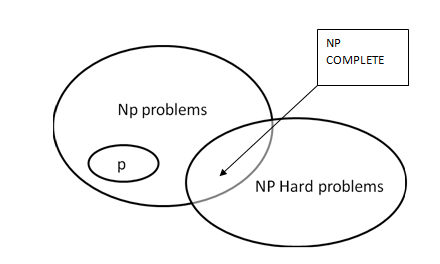
\includegraphics[scale=0.9]{np.png}\\
  \caption{Relation between Classes of Problems}
  
\end{figure}
\subsection*{\underline{Mathematical Model}}
 Let the proposed system be defined by set theory as:\\\\
S= $\{CLA , DC , PRED , PI , S , F , O , I , Q , q_0 , q_f , NDD , D , ALGO \}$ \\ \\
Where, \\ \\
I = input : $\{$ Voice commands through speech$\}$ \\ \\
O = output :$\{ $Services asked for in input speech in form of speech\}$ \\\\
$q_0$ = initial state: $\{$system starts and waits for the action keyword$\}$ \\\\
$q_f$ = final state: $\{$system speaks out the expected output to user$\}$ \\\\
S = success :$\{$ If the system works accurately without any halt or error.$\}$ \\\\
F = failure :$\{$System halts due to some error or doesn't perform functionality accurately.$\}$\\\\
Q = set of states:$ \{q_0, q_1, q_2, q_3, q_4, q_f\} $\\\\
D = deterministic data : $\{ Null\}$ \\\\
NDD = non deterministic data :$\{$ All states resulting output is non deterministic$\}$\\\\
CLA = classification : $\{ q_2:$ results in classified states or attributes of classes. $\}$\\\\
DC = data collection :$\{ q_1:$ results in data stored in Mongo Db $\}$\\\\
PRED = prediction: $\{q_4:$ results in expected output$\}$\\\\
PI = pattern identification :$\{ q_3:$ results in patterns as association rules$\}$ \\\\
\noindent
\textbf{Naive Bayes Time Complexity : }\\

The complexity of computing the parameters is  
$\Theta(\mid C \mid \mid V\mid)$ because the set of parameters consists of $\mid C \mid \mid V\mid$ conditional probabilities and $\mid C \mid$ priors. The preprocessing necessary for computing the parameters (extracting the vocabulary, counting terms, etc.) can be done in one pass through the training data. The time complexity of this component is therefore $\Theta(\mid D \mid L_{ave})$, where $\mid D \mid$ is the number of documents and $ L_{ave}$ is the average length of a document.\\


\textit{Table 3.1} summarizes the time complexities. In general, we have\\
 $\mid C \mid \mid V\mid < \mid D \mid L_{ave}$, so both training and testing complexity are linear in the time it takes to scan the data.  $ L_{a}$ and $ M_{a}$ are the numbers of tokens and types, respectively. Because we have to look at the data at least once, NB can be said to have optimal time complexity. Its efficiency is one reason why NB is a popular text classification method.\\

\begin{table}[ht]
\caption{Training \& Testing times for Naive Bayes}
\centering
\begin{tabular}{ |M{4cm}|p{7cm}|  }
 \hline
 mode & time complexity \\
 \hline
 training & $\Theta(\mid D \mid L_{ave} + \mid C \mid \mid V \mid)$\\
 \hline 
 testing & $\Theta(L_{a} + \mid C \mid M_a)=\Theta(\mid C \mid M_a)$\\
 \hline
 
 \end{tabular}

\end{table}
\vspace*{1cm}
\noindent
\textbf{Apriori Algorithm Time Complexity:}\\

Suppose the number of input transactions is N, the threshold is M, number of unique elements is R. The complexity for generating set of size i is $O(R\textsuperscript{$\wedge$}i)$ and the time for calculating support for each set can be done in O(n), if using HashMap. Therefore,  time complexity would be\\
\begin{center}
$O[(R + N) + (R\textsuperscript{$\wedge$}2 + N)  + (R\textsuperscript{$\wedge$}3 + N)  …] $\\
$= O[MN + (R\textsuperscript{$\wedge$}1+R\textsuperscript{$\wedge$}2+ … R\textsuperscript{$\wedge$}M)] $\\
$= O(MN+ (1-R\textsuperscript{$\wedge$}M)/(1-R))$
\end{center}



\newpage
\section*{\centering\LARGE{Lab Assignment 03}}
\subsection*{\underline{Aim}}
Use of divide and conquer strategies to exploit distributed/parallel/concurrent processing of the above to identify objects, morphisms, overloading in functions (if any), and functional relations and any other dependencies (as per requirements).
\subsection*{\underline{Concept}}
A divide and conquer algorithm works by recursively breaking down a problem into two or more sub-problems of the same (or related) type (divide), until these become simple enough to be solved directly (conquer). So have divided our problem based on algorithm used and those are:
\begin{itemize}
\item Data Collection.
\item Naive Bayes classifier for classifying (parallel computing used for calculating individual probabilities of the attributes).
\item Apriori algorithm for frequent pattern sets.
\item Decision tree for pattern identification.
\end{itemize}

\vspace*{0.4cm}
\noindent
\hspace{5em}Divide and conquer (D\&C) is an algorithm design paradigm based on multi-branched recursion. So we have to recursively divide our problem into  sub-problems  of the same (or related) type (divide), until these sub-problem become simple enough to be solved directly (conquer). The solutions to the sub-problems are then combined to give a solution to the original problem.\\

\vspace*{0.4cm}
\noindent
\hspace{5em}In our project we have divided our project into 4 phases which are : Data Collection, Data Classification, Pattern identification, and prediction. Now, in Data collection the data is stored as input for next step using a web crawler in a NOSQL database-MongoDB. Further for classifying data Naive Bayes classifier is used which classifies the crime type and its region of interest. Here parallelism will be used where  calculating the probabilities of Each and every class and attribute will be done in parallel.The classified classes are again stored in database and are used as input for next step. Next will be generating frequent pattern sets from the classified data Apriori algorithm. The last step will be generating patterns using decision tree.

\newpage
\noindent
\textbf{System Specifications and Dependencies}\\
The system comprises of following major components : 
\begin{itemize}


\item Data Collection using web crawler.
\item Data Classification using Naive Bayes classifier.
\item Generating frequent pattern sets using apriori algorithm.
\item Pattern identification using decision trees.
\end{itemize}

 \begin{figure}[H]
    \centering
  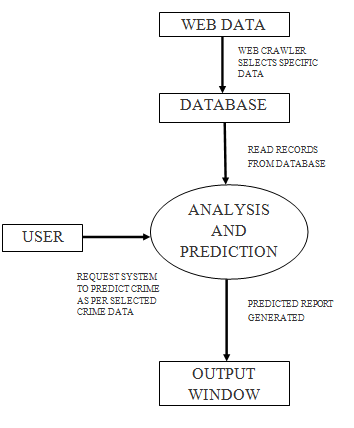
\includegraphics[scale=1.3]{DFDONE.png}\\
  \caption{DFD Level 1}
  
\end{figure}

    \begin{figure}[H]
    \centering
  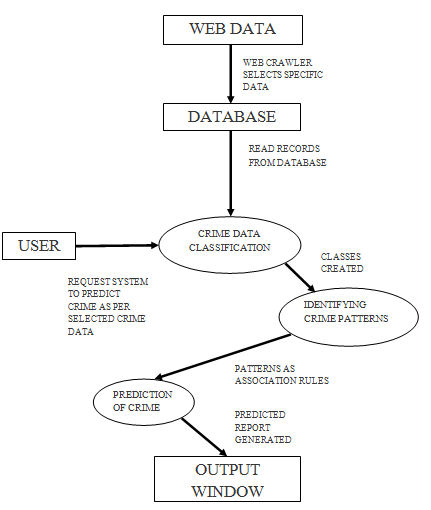
\includegraphics[scale=1.2]{DFDTWO.png}\\
  \caption{DFD Level 2}
  
\end{figure}
\newpage
\section*{\centering\LARGE{Lab Assignment 04}}
\subsection*{\underline{Aim}}
Use of above to draw functional dependency graphs and relevant Software modelling methods, techniques including UML diagrams or other necessities using appropriate tools.
    \subsection*{USE CASE DIAGRAM}
    \begin{figure}[H]
    \centering
  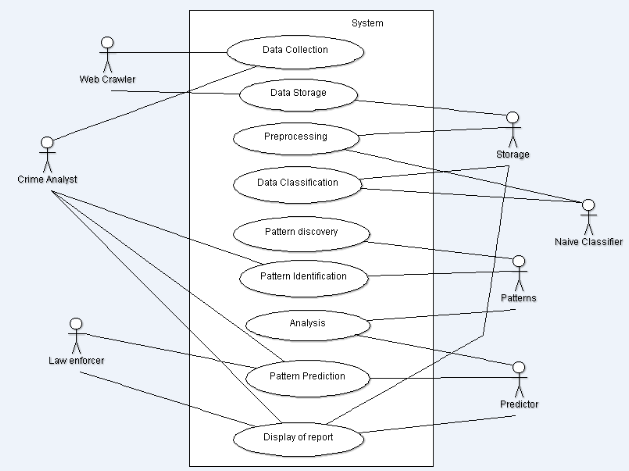
\includegraphics[scale=0.75]{USECRIME.png}\\
  \caption{Use Case Diagram}
  
\end{figure}
    \pagebreak
    \subsection*{DEPLOYMENT DIAGRAM}
     \begin{figure}[H]
  \centering
  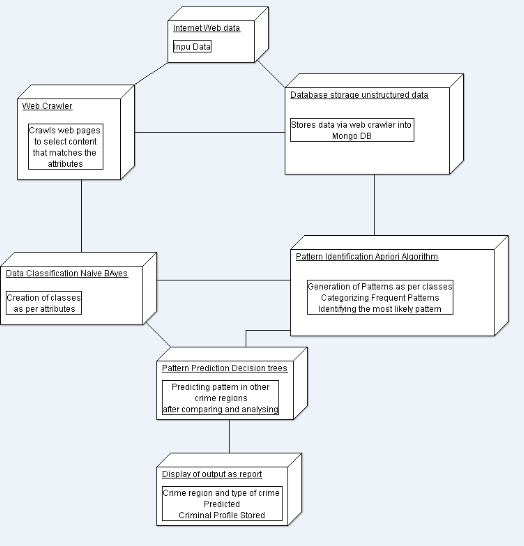
\includegraphics[scale=0.75]{DEPLOYDIAGRAM.png}\\
  \caption{Deployment Diagram}
  \end{figure}
  \pagebreak  
    \subsection*{ACTIVITY DIAGRAM}
    \begin{figure}[H]
  \centering
  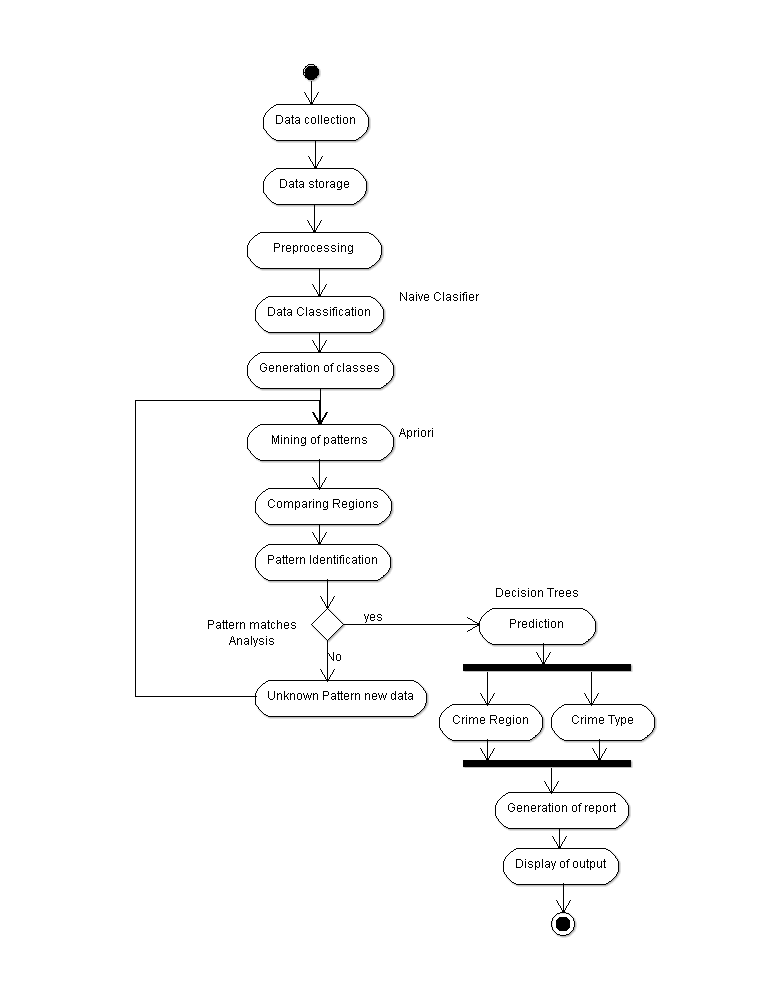
\includegraphics[scale=0.75]{ACTIVITYDIAGCRIME.png}\\
  \caption{Activity Diagram}
  
\end{figure}
    
   \pagebreak 
    \subsection*{SEQUENCE DIAGRAM}
    
    \begin{figure}[H]
  \centering
  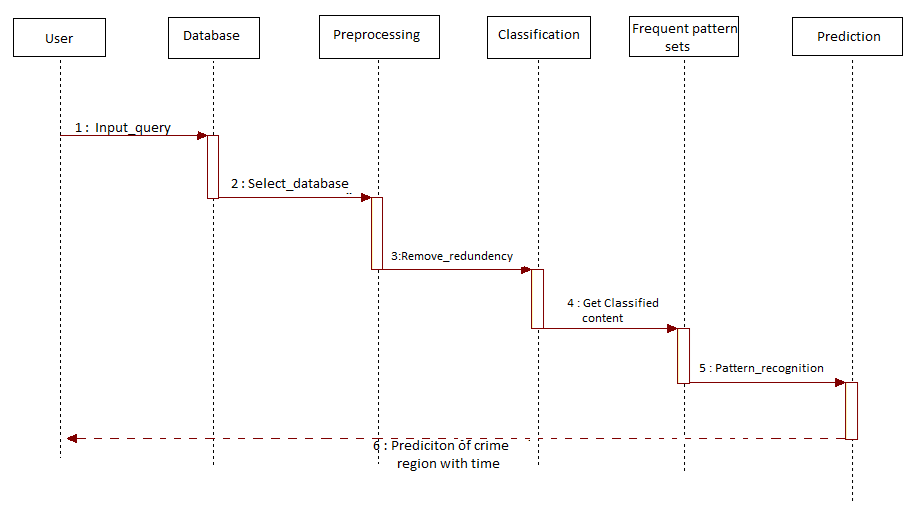
\includegraphics[scale=0.65]{SEQU.png}\\
  \caption{Sequence Diagram}
  
\end{figure}
 \pagebreak   
    \subsection*{STATE CHART DIAGRAM}
    
    \begin{figure}[H]
  \centering
  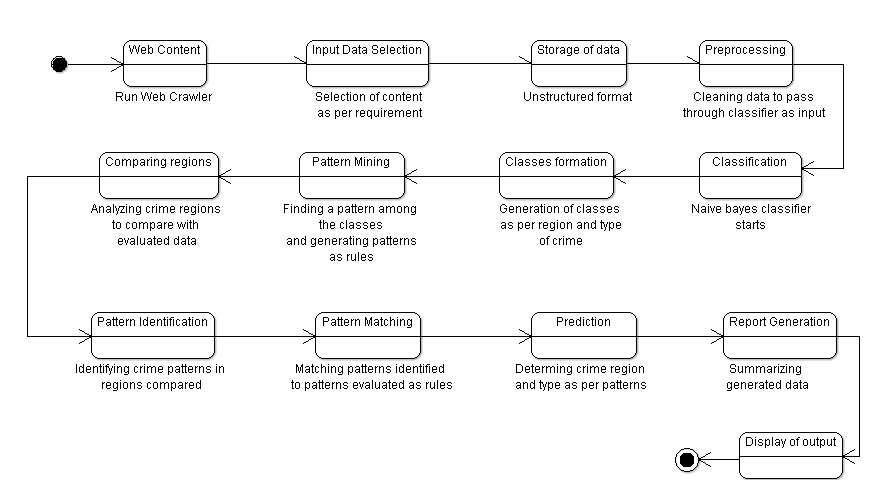
\includegraphics[scale=0.7]{STATECHARTCRIME.png}\\
  \caption{State Chart Diagram}
  
\end{figure}
\pagebreak
    \subsection*{CLASS DIAGRAM}
    \begin{figure}[H]
    \centering
  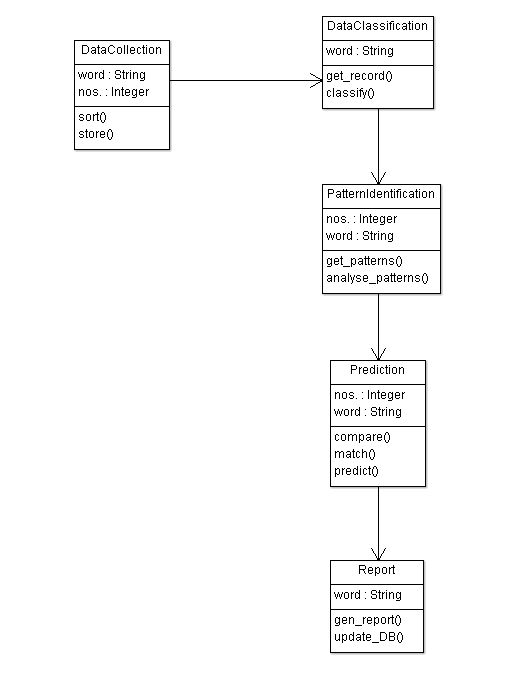
\includegraphics[scale=0.75]{CLASS.png}\\
  \caption{Class Diagram}
  
\end{figure}

\newpage
\section*{\centering\LARGE{Lab Assignment 05}}
\subsection*{\underline{Aim}}
Testing of project problem statement using generated test data (using mathematical models, GUI, Function testing principles, if any) selection and appropriate use of testing tools, testing of UML diagram's reliability.
\noindent
\subsection*{\underline{Testing}}
\hspace{5em}Testing is an investigation conducted to provide stakeholders with information about the quality of the product or service under test. Software testing also provides an objective, independent view of the software to allow the business to appreciate and understand the risks of software implementation. Test techniques include, but are not limited to, the process of executing a program or application with the intent of finding software bugs. Software testing can also be stated as the process of validating and verifying that a software program or application or product.\\

\noindent
\hspace{5em}Software testing, depending on the testing method employed, can be implemented at any time in the development process. However, most of the test effort occurs after the requirements have been defined and the coding process has been completed. As such, the methodology of the test is governed by the software development methodology adopted.In a more traditional model, most of the test execution occurs after the requirements have been defined and the coding process has been completed.


\subsection*{\underline{Testing types}}
It describes which testing types we might follow in our testing life cycle. Here we are using:
\begin{itemize}
\item \textbf{Black Box Testing}\\
Black box testing methods focus on the functional requirements in the software. That is, black box testing enables us to derive sets of input conditions that will fully exercise.\\
All functional requirements of the program Black box testing attempts to find errors in the following categories:
\begin{itemize}
\item Incorrect or missing function
\item	Interface errors
\item	Errors in data structure or external job access
\item	Performance errors
\item	Initialization and termination errors.
 
\end{itemize}

In the proposed application with the help of this technique, we do not use the code to determine a test suite; rather, knowing the problem that we are trying to solve, we come up with four types of test data: 
\begin{enumerate}
\item	Easy-to-compute data,
\item	Typical data,
\item	Boundary / extreme data,
\item	Bogus data.

\end{enumerate}
But in our application we does not provide any external data, the role of user is only to give number of nodes for formation of clusters and for the formation of sink node.


\item \textbf{White Box Testing}\\
White box testing is a set case design method that uses the control structure of the procedural design to derive test cases. Using white box testing methods, we can derive test cases that:
\begin{itemize}
\item 	Guarantee that all independent paths within a module have been exercised at least once.
\item	Exercise all logical decisions on their true and false sides.
\item	Execute all loops at their boundaries and within their operational bounds.
\item	Exercise internal data structures to ensure their validity.

\end{itemize}
In the proposed application the white box testing is done by the us on the implemented code, we study the code and then determines all legal (valid and invalid) and illegal inputs and verifies the outputs against the expected outcomes, which is also determined by studying the implementation code.


\item \textbf{Unit Testing}\\
Unit testing enables a programmer to detect error in coding. A unit test focuses verification of the smallest unit of software design. This testing was carried out during the coding itself. In this testing step, each module going to be work satisfactorily as the expected output from the module.
The front end design consists of various forms. They were tested for data acceptance. Similarly, the back-end also tested for successful acceptance and retrieval of data. The unit testing is done on the developed code. Mainly the unit testing is done on modules.

\item \textbf{System Testing}\\
After performing the integration testing, the next step is output testing of the proposed system. No system could be useful if it doesn't produce the required output in a specified format. The outputs generated are displayed by the user. Here the output format is considered in to two ways. One in on screen and other in printed format.


\item \textbf{Integration Testing}\\
Through each program work individually, they should work after linking together. This is referred to as interfacing. Data may be lost across the interface; one module can have adverse effect on the other subroutines after linking may not do the desired function expected by the main routine. Integration testing is the systematic technique for constructing the program structure while at the same time conducting test to uncover errors associated with the interface. Using integrated test plan prepared in the design phase of the system development as a guide, the integration test was carried out. All the errors found in the system were corrected for the next testing step.
\item \textbf{Functional Testing}

\item \textbf{GUI Testing}

\end{itemize}

\begin{table}[ht]
\caption{Test Cases}
\begin{tabular}{ |M{4cm}|p{5cm}|M{2.5cm}|M{3.2cm}|  }
 \hline
 \textbf{USE CASE} & \textbf{FUNCTION BEING TESTED} & \textbf{INPUT} & \textbf{EXPECTED OUTPUT}\\
 \hline
 
Data Collection & Is data collected properly? & Web data & Stored records in DB\\

\hline
 Data Classification & Is data classified into  classes as per attributes? & Data in DB & Classes of attributes\\
 
 \hline
 Pattern identification & Is unique patterns generated? & Classes from classifier & Patterns as rules.\\
 
 \hline
 Prediction & Is regions having a common pattern? & Rules from apriori & Expected output\\
  
  \hline
  
 
 \end{tabular}
 
\end{table}

